\documentclass[11pt, oneside]{article}
\usepackage{titling, hyperref, geometry, amsmath, amssymb, algorithm, graphicx, textcomp, subcaption, cancel}
\usepackage[noend]{algpseudocode}
\usepackage[cache=false]{minted}
\geometry{a4paper}

\hypersetup{
    colorlinks=true,
    urlcolor=cyan
}

\newcommand{\emphasis}[1]{\textcolor{blue}{\textbf{\textit{#1}}}}
\graphicspath{{./images/}}

\title{Suffix Trees and Arrays}
\author{Stephen Huan \\ Edited by: Udbhav Muthakana}

\begin{document}
\maketitle

\section{Suffix Trees}
\subsection{Trie}

\begin{figure}[h!]
\centering
\includegraphics[scale=0.25]{trie}
\caption{The trie data structure}
\end{figure}

A \emphasis{trie} is a tree based data structure that stores a list of strings.
Certain operations are faster with tries.

For example, consider the ``autocomplete'' problem of finding whether a given target string is a prefix of any of the pattern strings in a list.
Let \( T \) be the target string of length \( m \) and the pattern strings be \( P_1, P_2, \dots, P_k \).
We then define \( n \) to be \( \Sigma^{k}_{i = 1} |P_i| \), or the total length of all the pattern strings.
We propagate a pointer down the trie, following edge labels that correspond to characters in the target string.
If we ``fall off'' the trie - there aren't any more edges - then it isn't a prefix.
The notation I will use for running time is \( \langle f, g \rangle \),
where \( f \) is the preprocessing time and \( g \) is the query time.
For example, the naïve algorithm of scanning every pattern string
is \( \langle O(1), O(n) \rangle \), as it has no preprocessing time
but could scan every character in the patterns.
However, our trie algorithm yields an \( \langle O(n), O(m) \rangle \) algorithm,
which is asymptomically optimal, as reading the input string is already linear time.

Why is it important to find prefixes? Consider that a substring is always a prefix of a suffix.
First, we define a suffix by its starting index \( i \), such that the suffix \( i \)
is equal to all characters including and after \( i \) (i.e. \( s[i:] \)).
All substrings start at a given index and have a particular length.
The substring starting at \( i \) has the same starting point as the suffix \( i \) and a length less than or equal to that suffix's size, making the substring a
prefix of the suffix.
Therefore, all substrings are prefixes of suffixes.

If we want to determine whether a string \( T \) is a substring of another string \( P \),
we can compute it efficiently by determining whether \( T \) is a prefix of any suffix of \( P \).
This leads to the next data structure, a trie of all the suffixes of a particular string.

\subsection{Suffix Trie}

\begin{figure}[h!]
    \centering
    \begin{subfigure}[h]{0.4 \textwidth}
      \includegraphics[scale=0.25]{trie2}
      \caption{A trie}
    \end{subfigure}
    \hfill
    \begin{subfigure}[h]{0.4 \textwidth}
      \includegraphics[scale=0.25]{patricia}
      \caption{The resulting Patricia trie}
    \end{subfigure}
    \caption{A trie and its corresponding Patricia trie}
\end{figure}

First, we'll add an extra character to the end of the string,
``\$'' by convention (because it's lexicographically less than most characters),
so that no suffix is a prefix of any other suffix, which keeps the suffixes distinct.
Then, if we use our typical \( O(n) \) algorithm to generate a trie from all the suffixes of a string,
there are \( 1 + 2 + 3 + \dots + m = \frac{m(m + 1)}{2} \) total characters,
which is an \( O(m^2) \) time algorithm. However, note that some nodes are useless.
If a node only has one child, then there's only one path from it.
Therefore, we can ``compress'' adjacent so-called `silly nodes' into an edge,
which yields a \emphasis{Patricia trie} (or Radix trie).
This new structure has at most two nodes for each string added to the trie,
and thus can theoretically be constructed in \( O(m) \), because there are only \( m \) suffixes.
A Patricia trie of suffixes is known as a \emphasis{suffix tree}.

\subsection{Suffix Tree}

\begin{figure}[h!]
\centering
\includegraphics[scale=0.4]{tree}
\caption{A suffix tree}
\end{figure}

We arrive at our final data structure. The obvious use is substring matching,
but there are a variety of uses discussed in the sample problems at the end of the lecture.

To actually implement suffix trees, we can take advantage of several properties.
First, edges in the tree are substrings of the original string.
Thus, we'll represent an edge by its start and end indexes in the string.
Second, the edges emanating from a particular node must have unique first characters
(if they didn't, then there would be a new node).
Thus, we'll actually represent children via a dictionary, mapping the first character
of an edge to a node containing the start and end indexes that represent the actual edge.
This enables an O(1) lookup to determine whether or not to follow an edge in the tree.
Third, the leaves of the suffix tree correspond to suffixes.
We'll label leaves by the starting index of the suffix, as usual.
Lastly, we'll copy the original string and store the copy at the root of the tree,
in order to actually read what the edges say.

Certain properties of the suffix tree are important.
First, we say a node in the suffix tree ``corresponds'' to the string created by adding all of the edges to get to that node from the root.
The root corresponds to the empty string, commonly denoted \( \epsilon \).
Then, internal nodes in the suffix tree correspond to \emphasis{branching words} - substrings that appear in the string at least twice, with at least two of their occurrences being followed by distinct characters.
That is, a string \( \omega \) is branching if there exists at least two strings \( \omega a \) and \( \omega b \) that appear in the original string.

To prove this, we'll prove each direction. If a word is not branching, then it can't be an internal node.
A word isn't branching if it isn't in the string multiple times, or the same character is after each occurrence.
For the first case, it can't be an internal node since it doesn't have children.
For the second case, it's not an internal node because we can extend its edge by at least one character.
Now, we prove that if a node is an internal node, it corresponds to a branching word.
Since the node is internal, it must have more than one child (since we merge nodes with only one children together),
thus it repeats more than once. In addition, each of its children must have a distinct starting character,
thus a node is internal in a suffix tree if and only if it corresponds to a branching word.

The second interesting property is that since the leaves are suffixes, a sorted depth first traversal
(following lexicographically minimal edges first) will yield the suffixes in sorted order.
This brings us to our next data structure - an array of all the suffixes in sorted order, called a \emphasis{suffix array}.

\section{Suffix Arrays}

Suffix trees use too much memory for large strings (3-6 machine words per character).
Although this is a linear memory cost, consider human DNA, which is three billion characters long.
Normally, each character is a byte, but because DNA only has four different characters (A, C, G, T)
it's possible to have 1 nucleotide per 2 bits and thus 4 characters per byte.
Thus, DNA is 800 MB, which translates to nearly 96 GB of memory on a 64 bit machine
(far more than a typical computer can store).

\begin{figure}[h!]
\centering
\includegraphics[scale=0.25]{array}
\caption{A suffix array}
\end{figure}

Instead of storing a tree, we'll store an array of the suffixes in sorted order,
which only requires one word per character. Although the above diagram has strings,
we're actually storing integer starting positions as usual.

\subsection{Construction}

As previously mentioned, a DFS on a suffix tree yields a suffix array.
However, we'll actually construct the suffix array first, and use it to construct a
suffix tree later. The naïve algorithm is to use a standard \( O(n \log n) \) comparision based
sort on each suffix, but each comparision takes \( O(n) \) time and thus the entire algorithm
is \( O(n^2 \log n) \).

Instead, we'll construct suffix arrays by induced sorting (SA-IS).

\begin{figure}[h!]
    \centering
    \begin{subfigure}[h]{\textwidth}
      \centering
      \includegraphics[scale=0.4]{bucket}
      \caption{Each suffix bucketed by first character}
    \end{subfigure}
    \newline
    \begin{subfigure}[h]{\textwidth}
      \centering
      \includegraphics[scale=0.4]{label}
      \caption{Each suffix labeled as S-type or L-type}
    \end{subfigure}
    \caption{Bucketing and labeling applied to a string}
\end{figure}

First, we'll bucket each suffix by its first character.
This gives a pretty good preliminary sort, but we don't know the position of each
suffix in its bucket yet. Second, we'll label each index as \emphasis{S-type} or \emphasis{L-type}.
An index is S-type if the corresponding character in the string is lexicographically less than the index after it, or if it's the sentinel. An index is L-type if it's lexicographically greater. If the two are equal, then the index has the same type as the index after it.

\begin{figure}[h!]
\centering
\includegraphics[scale=0.4]{blabel}
\caption{Patterns under labeling and bucketing}
\end{figure}

We notice that in each bucket, the L-types come before the S-types.
This is because if an index is L-type, the character \textit{after} it is going to be smaller than it is.
Correspondingly, if an index is S-type, then the character after it is \textit{larger},
meaning L-type suffixes will always be lexicographically smaller than S-type suffixes in the same bucket.

Since we can bucket and label in \( O(n) \), we just need to sort the suffixes
within each group, i.e. suffixes with the same starting character and type.
We then define \emphasis{LMS suffixes}, or \emphasis{L}eft \emphasis{M}ost \emphasis{S}-type suffixes.
A suffix is a LMS suffix if it is S-type and the suffix before it is L-type.
The key observation is that if we can sort the LMS suffixes, we can
infer the sorted order of all other suffixes via ``induced sorting''.

\begin{figure}[h!]
    \centering
    \begin{subfigure}[h]{\textwidth}
      \centering
      \includegraphics[scale=0.35]{bbucket}
      \caption{Buckets with boundaries}
    \end{subfigure}
    \newline
    \begin{subfigure}[h]{\textwidth}
      \centering
      \includegraphics[scale=0.35]{lms}
      \caption{LMS suffixes}
    \end{subfigure}
    \caption{Buckets with boundaries containing the LMS suffixes in sorted order}
\end{figure}

\newpage

To see how this is possible, first determine the boundaries of each bucket by counting
how many times each character occurs in the string.
Then, put the LMS suffixes in sorted order from the right of the each bucket boundary.
Then, for each L-type suffix in order, put it at the front of its corresponding bucket.
Reset the rightmost bucket boundaries and then do a reverse scan of the S-type suffixes,
putting them at the back of each bucket and overwriting the existing LMS suffixes there.

The intuition behind this is that it simulates a multiway merge, but the details are rather messy and beyond the scope of this lecture.

However, we still need to sort the LMS suffixes. First, we define LMS blocks to be
the substring formed by starting from a particular LMS suffix to the next LMS suffix.


\begin{figure}[h!]
\centering
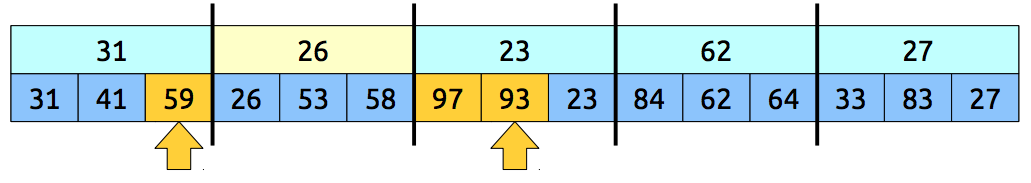
\includegraphics[scale=0.3]{block}
\caption{LMS blocks}
\end{figure}


Then, the order of the LMS suffixes depends on the order of their LMS blocks.
In order to sort LMS blocks, we can just put them into the buckets in an arbitrary manner (in order of appearance is easiest), and then run the aforementioned induced sort.

When we actually sort the LMS suffixes from the sorted LMS blocks, the problem is that LMS blocks end ``early'': before their corresponding suffix ends. However, note that a LMS suffix can be made up of multiple LMS blocks joined end to end.
Thus, sorting LMS suffixes is equivalent to rewriting the string as a sequence of LMS blocks.

\begin{figure}[h!]
\centering
\includegraphics[scale=0.4]{numbers}
\caption{LMS block numbers}
\end{figure}

Number each LMS block, giving the same block the same number
(check whether a block is equal to the one directly after it - when we sort the blocks, equal blocks have to be adjacent to each other).
We now have a new ``reduced string'', formed by adding block numbers in the order of when the LMS block appeared in the original string.
We number the LMS blocks because a smaller number will naturally be lexicographically smaller than a larger number,
and the suffix array of this new reduced string will sort the LMS suffixes
(since an LMS suffix is equivalent to its block plus all the blocks after it, which is represented in the reduced string).

\begin{figure}[h!]
\centering
\includegraphics[scale=0.3]{reduced}
\caption{The corresponding reduced string}
\end{figure}

We now run into a problem: the algorithm for finding a suffix array requires finding a suffix array.
However, we can resolve this seemingly paradoxical situation with recursion,
cleverly chosing a base case.

\newpage

\begin{figure}[h!]
\centering
\includegraphics[scale=0.4]{basecase}
\caption{The base case}
\end{figure}

If all the blocks are distinct, then the suffix array is the inverse of
the reduced string, i.e. if the index \( i \) corresponds to the number \( k \)
in the reduced string, then the index \( k \) is \( i \) in the suffix array (this inverse is called the \emphasis{rank array}).
Otherwise, we recur.

\begin{figure}[h!]
\centering
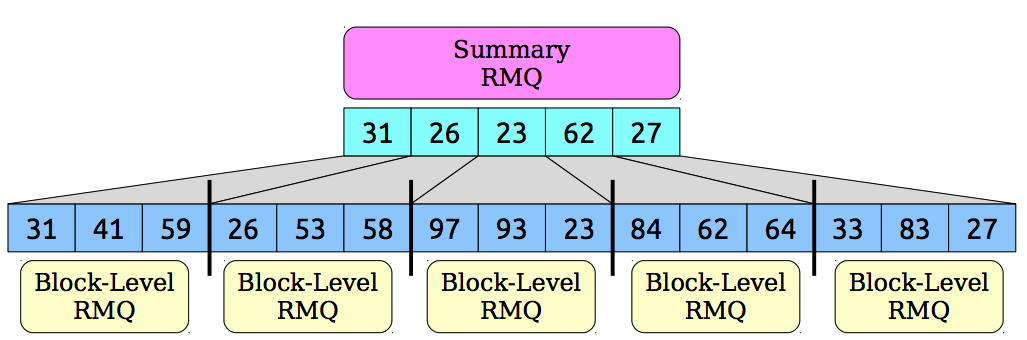
\includegraphics[scale=0.4]{summary}
\caption{Summary of SA-IS}
\end{figure}

The runtime of this algorithm is as follows:
first, the reduced string has to be at most half of the length of the original string,
since each LMS block is at least two characters (an S-type and an L-type), and each block
contributes one character to the reduced string.
Second, at each level of the recursion, the algorithm runs in \( O(n) \).
Then, the overall running time is \( O(n + \frac{n}{2} + \frac{n}{4} + \frac{n}{8} + \dots + 1) \).
Since the geometric series \( 1 + \frac{1}{2} + \frac{1}{4} + \dots \) converges to 2,
then the algorithm runs in \( O(2n) = O(n) \).

One nontrivial implementation detail is to convert the string from a list of characters
to a list of integer ASCII values. This prevents character overflow (possible in C++)
and is more convenient overall, as the reduced string and the original string are both lists of integers.
If you keep them as strings, then if there are more than ten blocks, the number will have two digits
and thus will not be represented in one character. However, this won't happen with integers.

A sample implementation in Python is given \href{https://gist.github.com/stephen-huan/aa609965c86d750736398c28b025f9be#suffix-array}{here}
along with all other algorithms discussed in this lecture.
An alternative C++ implementation is given \href{https://gist.github.com/stephen-huan/d660e04476f06695663401d0ac01a27a#suffix-array}{here}.

\section{LCP Array}

Our linear time suffix array is all well and good, but a plain suffix array can't replace a suffix tree.
As previously mentioned, the leaves of a suffix tree correspond to suffixes, and the internal nodes correspond to branching words.
The suffix array gives us the leaves, but what about internal nodes?

We define the \emphasis{L}ongest \emphasis{C}ommon \emphasis{P}refix (LCP)
to be the length of the longest common prefix.
For example, the LCP between ``abcd'' and ``abef'' is 2.

\begin{figure}[h!]
\centering
\includegraphics[scale=0.25]{lcp}
\caption{LCP array}
\end{figure}

The \emphasis{LCP array} is then the LCP values between adjacent suffixes in the suffix array.
Note that the LCP value corresponds to the \emphasis{string depth}
(the length of a node's corresponding string)
of the lowest common ancestor (LCA) between the two leaves in the suffix tree,
since in a trie, parents are the longest possible prefixes of their children.

\subsection{Construction}

Luckily, the algorithm to construct a LCP array is relatively simple compared to SA-IS.
First, consider the LCP value \( h \) between a particular suffix \( i \)
and the suffix \( k \) immediately before it in the suffix array.
If you then consider the suffix after \( i \), \( i + 1 \), then that suffix must
have an LCP of at least \( h - 1 \) with its adjacent suffix, because \( i \) and \( i + 1 \)
have the same prefix with one character removed from \( i + 1 \). Thus, the
suffix \( k + 1 \) matches with \( i + 1 \) for at least \( h - 1 \) characters.

In order to find the position of a suffix in the suffix array, compute the rank array.
Then, we start with the longest suffix, or the suffix at index 0.
Compute \( h \) between the suffix 0 and its adjacent suffix by the naïve algorithm: start at \( h = 0 \) and check whether s[i + h] == s[k + h], incrementing \( h \) if they are.
From our previous observation, the next suffix of \( i + 1 \) has to match with its adjacent suffix
at least \( h - 1 \) characters, thus we can decrement the current value of \( h \)
by 1 and start checking from there. This algorithm is called \emphasis{Kasai's algorithm} and runs in \( O(n) \) - \( h \) must be less than \( n \), the length
of the string, and decreases at most \( n \) times, thus \( h \) changes value
at most \( 3n \) times.

\subsection{Non-pairwise LCP}

The LCP array only stores the LCP value for adjacent suffixes.
How do we generalize to the LCP between any two suffixes?

The key observation is that the LCP value between two nonadjacent suffixes
is the minimum LCP value between them in the LCP array.
To see why, notice that LCP decreases monotonically when moving away from a suffix.
Since the suffix array is sorted lexicographically, suffixes with a larger LCP
value must be closer to a particular suffix than suffixes with a smaller LCP value.
Call the LCP value \( h \) and the minimum LCP value between the two suffixes \( m \).
\( h \leq m \) because of monotonicity.
Also, \( h \geq m \) because a range minimum of \( m \) implies there exists a prefix of length \( m \)
common to all suffixes between the two suffixes, making the LCP at least \( m \).
If \( m \leq h \leq m \), then \( h = m \).

Thus, we can construct an \( \langle O(n), O(1) \rangle \) range minimum query (RMQ) structure
on the LCP array (most likely Fischer-Heun).
Then, the LCP between two suffixes \( i \) and \( j \) is lcp[rmq(lcp, i, j - 1)] assuming \( i \leq j \), an \( O(1) \) query.

\section{Constructing Suffix Trees}

We've seen how both suffix arrays and LCP arrays can be constructed in \( O(n) \). \\
How do we construct suffix trees in \( O(n) \)?

There exist direct algorithms like Ukkonen’s, but we'll use a more indirect method.
First, recall that an inorder DFS of the suffix tree results in the suffix array.
Second, recall that the LCP value corresponds to the string depth of a node in the suffix tree.
These two observations inspire Cartesian trees.
A \emphasis{Cartesian tree} is defined as a binary tree whose inorder traversal yields the original array and is a min-heap.

Notice how the two properties of a Cartesian tree aligns with properties of the suffix tree.
If we build a Cartesian tree on the LCP array, then the inorder traversal of the Cartesian tree
will yield the LCP array, which corresponds to suffixes.
In addition, within the same subtree, larger string depth implies larger height.
Thus, the min-heap property guarantees that in the same subtree, greater LCP values are lower in the tree.

\begin{figure}[h!]
\centering
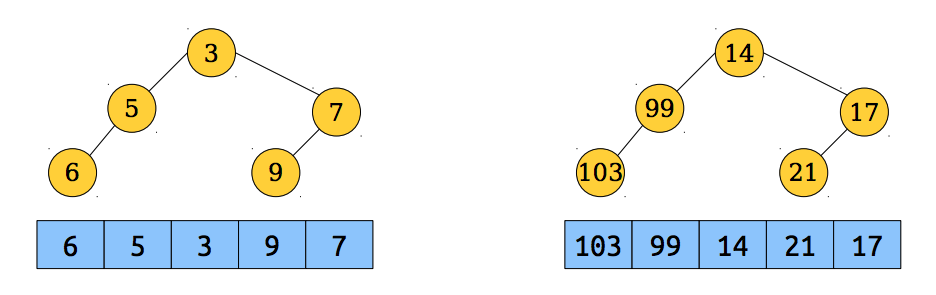
\includegraphics[scale=0.19]{cartesian}
\caption{Cartesian tree built on the LCP array}
\end{figure}

\begin{figure}[h!]
\centering
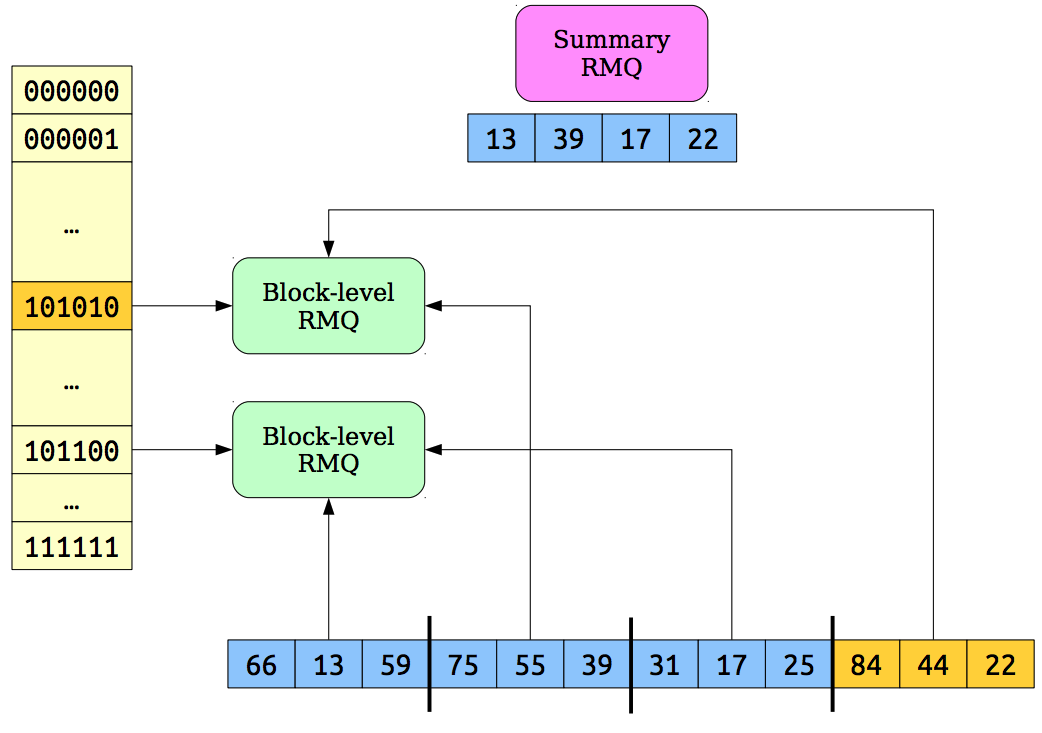
\includegraphics[scale=0.25]{final}
\caption{Suffix tree formed by merging nodes}
\end{figure}

Merge nodes with the same LCP values into their parents before labeling edges.

\begin{figure}[h!]
\centering
\includegraphics[scale=0.25]{edge}
\caption{Cartesian tree with labeled edges}
\end{figure}

DFS on the Cartesian tree, adding suffixes as children to nodes missing children.
Then, label edges based off the LCP values.
Recall that edges are represented by a start and end index, and that
suffixes start at their index and end at the end of the string.
A node will end at the minimum start of its children minus 1,
and will begin at its end minus the difference in LCP between it and its parent
(the length of the edge).

\section{Generalizations}
\subsection{Generalized Suffix Arrays}

The suffix structures we've discussed up to this point only apply to a single string. \\
What about multiple strings?

Luckily, suffix arrays generalize extremely easily.
Simply concatenate all the strings together, with a unique delimiter in between them.

\begin{minted}{python}
def generalized_suffix_array(words: list) -> tuple:
    n = [v for i, word in enumerate(words) \
         for v in (list(map(ord, word)) + [i - len(words)])]
    return n, suffix_array(n)
\end{minted}

\subsection{Generalized Suffix Trees}

\begin{figure}[h!]
\centering
\includegraphics[scale=0.4]{general}
\caption{A generalized suffix tree}
\end{figure}

Creating a generalized suffix tree takes more work.
Keep track of a mapping from every suffix to the string it belongs to
and from a string to its starting position in the concatenated string.
Then, we have to prune out suffixes by ending them at their own string's delimiter, rather than the end of the concatenated string.

The resulting algorithm is to, as before, concatenate all the strings together with a unique delimiter in between them.
Create a suffix tree, and instead of suffixes ending at the end of the concatenated string, they should end at the start of the next word.

\newpage

\section{Sample Problems}

\begin{enumerate}
  \item \href{https://www.spoj.com/problems/SARRAY/}{SPOJ SARRAY}:
  Construction of suffix array.

  \item \href{https://www.spoj.com/problems/DISUBSTR/}{SPOJ DISUBSTR}:
  Given a string \( s \) with length \( m \), find the number of distinct substrings.
  For example, ``aab'' has 5 (``a'', ``b'', ``aa'', ``ab'' and ``aab'').

  Solution: In order to count the number of distinct substrings,
  we will first find the total number of substrings and then subtract out duplicates.
  The total number will be \( m \) substrings of length 1, \( m - 1 \) substrings of length 2,
  \( \dots \) \( 1 \) substring of length \( m \). \( 1 + 2 + 3 \dots + m \) equals
  \( \frac{m(m + 1)}{2} \) substrings.

  Recall that a substring is a prefix of a suffix. Build a suffix array
  and an LCP array, and think of each suffix as a starting point for
  possible substrings. Then, the number of duplicates for a particular suffix is the greatest
  longest common prefix (the LCP!) for any other suffix. This would seem like an \( n^2 \) loop:
  for each suffix, for each other suffix, find the LCP value and return the largest one.
  However, recall that the LCP between two suffixes is the minimum of adjacent LCP values.
  Therefore, LCP values must monotonically decrease, and the largest LCP value for a particular suffix is in the precomputed LCP array. Therefore, the number of duplicates will be just the sum of the LCP array.

  \item \href{https://www.spoj.com/problems/MINMOVE/}{SPOJ MINMOVE}:
  Given a string \( s \), find its lexicographically minimal cyclic \\ rotation,
  breaking ties by the starting index of the rotation.

  Solution: Think of a cyclic rotation as starting at some index \( i \).
  A rotation is then formed by adding the the prefix of \( s \) ending at \( i \) to the suffix of \( s \) starting at \( i \).
  We can sort rotations by their suffix half with suffix arrays, and then pick the first suffix, disregarding the special terminator ``\$''
  (suffix arrays are lexicographically sorted by definition, so the minimum suffix appears first in the suffix array). However, this doesn't sort rotations by prefix.
  For example, take the string ``dbcz\textcolor{green}{b}cd\textcolor{red}{b}c''.
  The algorithm might compare the suffix at index \textcolor{red}{7}, ``bc'', with the suffix at \textcolor{green}{4},
  ``bcdbc'', and conclude that ``bc'' \( < \) ``bcdbc'' without checking the entire rotation,
  and after looking at ``bcdbc\emphasis{z}'' and ``bcdbc\emphasis{d}'',
  the suffix at 4 actually wins. To account for this, add the string to itself.
  Since the latest possible rotation occurs at the length of the string, all rotations
  finish within two times the length of the string. Therefore, the string doubled will
  allow each rotation to be completely compared. Going back to the previous example,
  the resulting string is ``dbcz\textcolor{green}{b}cd\textcolor{red}{b}cdbczbcdbc'', and the suffixes are correctly compared.

  However, doubling adds two complications. First, only suffixes that occur in the first half of the string
  actually correspond to valid rotations. Second, for two suffixes that are identical (take the example of ``aaa''),
  the algorithm will take the shorter suffix, which corresponds to a greater index. The solution is to add a character
  lexicographically greater than any other character to the end of the string, forcing greater index suffixes to the right in the suffix array.

  The final algorithm is to take \( s \), add it to itself, add a character
  (I pick ``\{'' for its ASCII value greater than ``z'''s), and then add the standard ``\$'' to terminate the string.
  Build a suffix array on this new string, and then scan from left to right,
  returning the first suffix which is less than the length of the string.

  \item \href{https://www.spoj.com/problems/BEADS/}{SPOJ BEADS}:
  Identical to the previous problem, with the annoyance of 1-indexing.
  The ``doubling'' solution actually times out for me, motivating another solution.

  Prepare the LCP array for \( O(1) \) RMQ as discussed above. We again scan the suffix array
  from left to right, although we will compare suffixes without doubling. We only need to
  compare suffixes if one is a prefix of another - if this is not the case,
  then there is a character on which they differ, making one unambiguously greater than the other.
  Otherwise, one suffix beats the other on length, which may not be correct for rotations.
  Find \( h \), where \( h \) is the LCP value between the current best suffix, \( b \), and a new suffix, \( i \).
  Check if \( h \) is equal to the length of one of the suffixes. If it is, then we need to compare
  the prefixes of the two suffixes. Since a prefix is lexicographically less than the original string,
  \( b \) is guaranteed to be shorter than \( i \), and thus ``wraps around'' \( s \) first. In order to compare
  \( b \) and \( i \), find the latest point either of them shares characters and compare the character after that point.
  \( i \) shares \( h \) characters with \( b \), so we start \( i \) at \( i + h \) and compare it to the start of \( s \), which is the suffix starting at 0. Compute \( p \), the LCP value between suffixes \( i + h \) and 0. \( i \)'s comparison point is then \( (i + h + p) \mod (|s| - 1) \) (modulo because rotations wrap around \( s \), minus 1 because \( s \) ends with ``\$''), and  \( b \)'s point is  \( p \).
  Therefore, if \( s[ (i + h + p) \mod (|s| - 1)] <= s[p] \), update \( b \) to \( i \).

  \item \href{https://open.kattis.com/problems/burrowswheeler}{Kattis burrowswheeler}:
  Compute the Burrows-Wheeler transform of a given string. The Burrows-Wheeler
  transform (BWT) of a string is defined by generating all cyclic rotations and
  then going through the rotations in lexicographic order, constructing a new string
  from the last character in each rotation.

  Solution: We already know how to sort cyclic rotations of a string from the aforementioned
  ``doubling'' algorithm. There are two complications:
  \begin{enumerate}
    \item We need the last character of each rotation. If a rotation starts at index \( i \),
    then its last character is \( i - 1 \mod n \).
    \item Most online sources claim sorting cyclic rotations can be done with just \\ s[SA[i] - 1],
    but this is assuming the string ends with a unique delimiter.
  \end{enumerate}

  \item \href{http://www.spoj.com/problems/BWHEELER/}{SPOJ BWHEELER}:
  Given the BWT, recover the original string.

  A simple algorithm is given \href{https://www.cs.helsinki.fi/u/tpkarkka/opetus/12s/spa/lecture11.pdf}{here} (no relation to suffix structures).

  \item \href{https://www.spoj.com/problems/LPS/}{SPOJ LPS}:
  Given a string \( s \) of length \( n \), find the length of the longest substring that is palindromic. A string is palindromic if it's equal to its reverse.

  Solution: The reverse of \( s \), denoted \( s' \), might be useful, because a palindrome of \( s \)
  will also appear in \( s' \). However, we can't just find the longest common substring
  between \( s \) and \( s' \) - take the example of ``abdeba'' and the reverse ``abedba''.
  The longest common substring between the two is either ``ab'' or ``ba'', but the longest palindrome
  is one character long. Therefore, we'll need to decompose palindromes in another way.

  Think of a palindrome as having a ``center'' index and a ``radius''.
  The palindrome starts at some center, and extends in either direction the radius number of characters.
  For example, the palindrome in ``dfe\emphasis{abba}g'' has a center of 5 and a radius of 2.
  Thus, to find the longest palindrome, go through each center and find the largest radius at that center.
  The largest radius is equal to the length of the longest string that occurs before and after the center,
  and since we have the reverse string, \( s' \), it's equal to the longest string after the center
  and after the position of the center in \( s' \)
  (a character on the left side of \( s \) appears on the right side of \( s' \)).
  In order to calculate that, create a generalized suffix array on \( s \) and \( s' \),
  and then compute the LCP array. Prepare the LCP array for constant time RMQ, and
  now the longest prefix of two suffixes is just the LCP value between them.

  Odd length palindromes (like ``aca'') are computed similarily - just offset the ``reverse position'' by 1.

  \item \href{https://leetcode.com/problems/longest-palindromic-substring/}{Leetcode LPS}:
  Equivalent to the previous problem, but return the palindrome.

  Keep track of the starting index \( i \) along with the size \( l \) of the longest palindrome.
  Return the substring \( s[i - \lfloor \frac{l}{2} \rfloor: i + \lceil \frac{l}{2} \rceil] \) (the radius is symmetric to the center).

  \item \href{https://leetcode.com/problems/palindromic-substrings/}{Leetcode palindromic-substrings}: Count the number of palindromic substrings.

  Since palindromicity is monotonic, finding that the longest palindrome has a radius of
  \( R \) implies that the center also has valid palindromes of radius \( r = 1, 2, 3, \dots, R \).
  Use the aforementioned algorithm, but add up the radii instead of finding the max.

  \item \href{https://www.spoj.com/problems/STAMMER/}{SPOJ STAMMER}/\href{https://contest.usaco.org/DEC06.htm}{USACO Gold December 2006 Milk Patterns} (\href{http://poj.org/problem?id=3261}{POJ link}): \\ Direct application of longest \( k \)-th repeated substring.

  Solution: Build a suffix tree on the string. Then, a substring will repeat \( k \) times
  if it has at least \( k \) leaves in its subtree. Run a DFS on the suffix tree, counting
  the number of leaves under each node and maintaining the string length up to that node.
  Pick the node with the largest string length that has at least \( k \) occurrences.

  \item \href{https://www.spoj.com/problems/LCS/}{SPOJ LCS}/\href{http://www.spoj.com/problems/ADAPHOTO/}{SPOJ ADAPHOTO}:
  Direct application of longest common substring.

  Solution (using suffix arrays): Construct a generalized suffix array on the two strings.
  Then, substrings which appear in both strings must be adjacent in the suffix array and
  have length equal to the LCP of the two suffixes.
  Scan through the suffix array, and if the pair is valid (each suffix starts in a different string)
  then consider whether the LCP value between them is larger than the current best.

  This can apparently be generalized to multiple strings in \( O(n) \)
  if one is somehow able to determine whether a range contains suffixes from all of the strings in \( O(1) \)
  and keep track of the minimum LCP value in a range using a sliding window technique with a structure like a monotonic queue.

  \item \href{https://www.spoj.com/problems/LONGCS/}{SPOJ LONGCS}/\href{http://www.spoj.com/problems/LCS2/}{SPOJ LCS2}:
  Direct application of LCS for more than two strings.

  Solution (using suffix trees): Construct a generalized suffix tree on all the strings.
  Then, valid substrings must have leaves from all the strings
  and have lengths equal to the string depth up to that node. Run a DFS on the suffix tree,
  numbering each leaf based on which string it came from, counting the number of distinct IDs under each node, and maintaining the string length up to that node.
  Pick the node with the largest string length that contains all strings.

  How do you count the number of distinct IDs under a node, given that each leaf has an ID?
  The count for a particular node will be the sum of the count of each of its children, minus duplicates.

  To keep track of the number of duplicates, consider two leaf nodes. Any node lower than the LCA
  of these two leaves will not have one of them in its subtree and thus will not have duplicates resulting
  from these leaves, and any node higher than the LCA is inductively corrected if the LCA is correct.
  Therefore, you only need to subtract one from the count of the LCA.

  The final algorithm: while running the DFS, keep track of the last leaf node seen for each ID.
  On processing a leaf node, subtract one from the LCA of the current node and the last node seen.
  For a non-leaf node, add up the counts of its children.

  \item \href{http://www.usaco.org/index.php?page=viewproblem2&cpid=768}{USACO Platinum December 2017 Standing Out from the Herd}

\end{enumerate}

\newpage

\section{Future Work}
Here I have given a fairly comprehensive view of string data structures - tries,
Patricia tries, suffix trees, generalized suffix trees, suffix arrays, and the LCP array. While not covered here, I and others have written SCT lectures on string matching,
using structures like the Aho-Corasick finite state automaton.

However, I have left out suffix automata. Perhaps that is room for future lectures?

\section{Past Lectures}

\begin{enumerate}
  \item \href{https://activities.tjhsst.edu/sct/lectures/1819/2019_03_29_Suffix_Arrays_and_LCP.pdf}{``Suffix Arrays and Longest Common Prefix'' (Daniel Wisdom, 2019)}
  \item \href{https://activities.tjhsst.edu/sct/lectures/1819/2018_12_07_Suffix_Arrays.pdf}{``Suffix Arrays and SA-IS'' (Charlie Gunn, 2018)}
  \item \href{https://activities.tjhsst.edu/sct/lectures/1617/2017-05-24_Suffix_Arrays.pdf}{``Suffix Arrays'' (Justin Zhang, 2017)}
\end{enumerate}

\section{Works Cited}

\begin{enumerate}
  \item Stanford lectures
    \begin{enumerate}
      \item \href{http://web.stanford.edu/class/cs166/lectures/02/Slides02.pdf}{Suffix Trees}
      \item \href{http://web.stanford.edu/class/cs166/lectures/04/Small04.pdf}{Constructing Suffix Arrays and Trees}
      \item \href{http://web.stanford.edu/class/cs166/lectures/03/Slides03.pdf}{Constructing LCP array}
      \item \href{http://web.stanford.edu/class/archive/cs/cs166/cs166.1186/lectures/03/Small03.pdf}{Applications of Suffix Trees}
      \item \href{http://web.stanford.edu/class/cs97si/suffix-array.pdf}{Suffix Trees in Competitive Programming}
      \item \href{https://web.stanford.edu/class/cs262/presentations/lecture4.pdf}{Burrows-Wheeler}
    \end{enumerate}
  \item \href{https://github.com/vladtepes1473/FM-Index/blob/master/readings/Linear%20Suffix%20Array%20Construction%20by%20Almost%20Pure%20Induced-Sorting.pdf}
  {Original paper on SA-IS}
  \item \href{http://web.cs.iastate.edu/~cs548/references/linear_lcp.pdf}{Original paper on Kasai's algorithm for LCP}
\end{enumerate}

\end{document}
